Modeling temporal data is of great interest in numerous branches of science.
Since the passage of time is so deeply embedded in our experience of the world, 
it is understandable that many scientific questions are posed in a \emph{dynamic}
setting. Arguably, the very concept of life implies variation in time and so 
as an example of a dynamic system we can consider any biological being, such as ourselves.
Measuring heart rate or neuronal activity or any \emph{biosignal}, 
with any of the available technologies,
produces sequential data \parencite[see, e.g.,][for a recent application]{Sarkka2012}. A
classic example of a dynamic
system is \emph{target tracking}, where based on a sequence of 
noisy range or angular measurements from a measurement intrument, typically a radar, 
we would like to continuously 
estimate the true position and velocity of the target \parencite{bar2004estimation,Godsill2007}. 
%This is understandable, since natural organisms inhabit a dynamic environment and
%it is natural organisms, such as ourselves, that easily draw our attention and raise questions
%deserving a scientific answer. The accuracy of the predictions, based on earlier observations,
%is indeed a property that can easily affect the survival of the forecaster.  

%Causality and consequences of actions are concepts tied to the passage of time.
%It should be noted that sequential data does not imply variation in \emph{time}.
%The variation might take place along any other unidimensional attribute,
%such as distance or order. Without loss in generality, in the sequel the notation 
%is derived by assuming variation in time. 

Let us assume the existence of a sequential dataset which is a result of 
making \emph{measurements} on a \emph{system} of interest. In order to answer questions of interest
about the system quantitatively,
the system and the measurements should be mathematically \emph{modeled}. The class of mathematical
models for dynamical systems we will be concerned with are known as \emph{state space models} (SSMs).
Important characteristics of SSMs are \emph{stochasticity} and decoupling of the system dynamics and the
measurements. At any instant, the system is thought to be in a certain finite-dimensional \emph{state}. The state
summarizes enough information about the system so that it is possible to formulate the system
state at the next instant as a function of the current state and \emph{process noise}.  
However the state is \emph{hidden} (or \emph{latent}) and the inference on the state has 
to be made entirely based on the measurements.  Often some components of the measurements 
would otherwise translate directly to corresponding components of the state, except that 
the measurements are always assumed to be \emph{noisy}.
As an example, in target tracking the state should contain at least the location and 
the velocity of the target. 

The stochasticity forces us to assume a probabilistic framework. In this thesis the viewpoint
is decidedly \emph{Bayesian}. In Bayesian statistics, ideally, the complete answer
is always the \emph{posterior probability distribution}, meaning the joint probability distribution
of the random variables of interest given the measurements. Thus instead of answering
with a single value or a value with error bounds, the answer is the probability
density function of the interesting quantity given the data. It is important to highlight,
however, that Bayesian statistics can be used to treat many kinds of uncertainty
\parencite[as pointed out in e.g.][]{Sarkka2012a}. For example, the instruments used 
to obtain the measurements are a source of uncertainty related to randomness, 
whereas our uncertainty regarding the model and its parameters implies
another kind of uncertainty. Both kinds of uncertainties can be quantified with Bayesian
statistics and thus applying statistical methods to a problem does not imply that the problem 
is actually random.

SSMs are a general framework and in any specific application prior knowledge of the
system has to be brought in. This prior knowledge is not necessarily very specific,
for example in ballistic target tracking it might include the assumption that Newton's
laws are applicable. The mathematical form of the dependence
between the measurements and the state has to be formulated as well as the dependence
of the state on its predecessors. Usually one is able only to specify the 
\emph{parametric} form for these equations. This results in a model with a set
of unknown parameters, denoted with $\Th$. In the Bayesian framework, $\Th$ is
a random variable with some prior probability distribution $\Pdf{\Th}$.
In order to complete the model, $\Th$ needs to be estimated based on some available
training data, the same sequential dataset we assumed earlier. This is sometimes, at least
in control engineering, known as \emph{system identification}. In this thesis,
it is assumed that the parameters are static, that is independent of time. 
This is then an important distinction between the states and
the parameters, in this thesis.

In general, assuming the aforementioned distinction between parameters and states, there are two separate but
interconnected estimation problems in SSMs: that of the states and that of the parameters. 
The interest might lie in either one or both, depending on the model. Traditionally, state
estimation, given measurements up to the current instant, is known as \emph{filtering}.
The term can be thought to relate to the idea of filtering the noise out of the measurements
in order to observe the states. Given a batch of measurements, state estimation is called \emph{smoothing}.
In order to engage in smoothing, the batch of measurements needs to be collected in its entirety, 
making smoothing an \emph{offline} procedure. Filtering, on the other hand, is \emph{online}, 
meaning the estimates can be updated every time a new measurement arrives.

A distinction is drawn in this thesis between \emph{linear} and \emph{nonlinear}
models. The linear model can be thought of as a special case of the nonlinear model,
so that linear models could be implicitly covered by only considering nonlinear models.
The distinction is useful for the simple reason that in the linear case closed
form solutions exist. The Bayesian solution of the filtering problem for a linear system
with additive Gaussian noise is given by the celebrated \emph{Kalman filter} \parencite{Kalman1960}.

Our focus in this thesis is in the static parameter estimation problem for the nonlinear case.
Depending on the method, this requires either the filtering or filtering and smoothing
solutions of the state estimation problem. Thus the state and parameter estimation problems
are inherently connected. For reasons of computational
complexity, we will not try to pursue the complete Bayesian solution of finding the 
posterior distribution. We will settle for a point estimate called the 
\emph{maximum a posteriori} (MAP), which is the mode (the value of the parameter giving the maximum) 
of the posterior distribution \parencite{gelman2004}.
Under an assumed \emph{uniform} prior distribution, the MAP estimate becomes equivalent 
with the \emph{maximum likelihood} (ML) estimate. The philosophical difference between these 
two might be fundamental, but as will be seen, from the perspective of the estimation equations it is not.

Figure~\ref{fig:ar1} illustrates the concepts of states, measurements and parameters. In
Figure~\ref{fig:ar1_simulation}, we have simulated a simple first order autoregressive (AR(1)), or first order
\emph{random walk}, model for $T=150$ steps. The states, $x_k$, are unidimensional and are denoted with a continuous
line. This reflects the fact, that commonly the system of interest operates in \emph{continuous}
time. The measurements, $y_k$, are denoted with crosses which reflects the fact the 
measurements, our sequential dataset, are almost always discrete. The model in Figure~\ref{fig:ar1}
has a parameter $\theta$ and the simulation
in Figure~\ref{fig:ar1_simulation} is made with $\theta=1$. In Figure~\ref{fig:ar1_lh}, we have
tried to estimate $\theta$, based only on the measurements. We have drawn a curve, which
can be described as the likelihood function or the unnormalized posterior probability distribution
with a uniform prior distribution. We can see that if we choose as our estimate the mode 
of this curve, denoted with a star, our estimate would be close to the true value. 
%
% 
\begin{figure}[htb]%
    \centering%
    %\makebox[\textwidth]{%
    \begin{subfigure}[t]{0.5\textwidth}%
    	\caption{}\label{fig:ar1_simulation}%
    	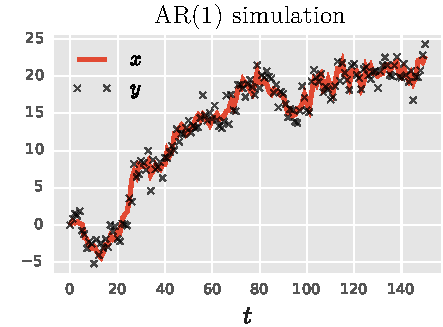
\includegraphics{img/ar1_ex_a}%
    \end{subfigure}%
    \begin{subfigure}[t]{0.5\textwidth}\centering%
		\caption{}\label{fig:ar1_lh}%
		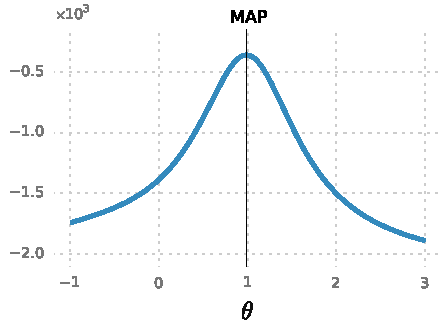
\includegraphics{img/ar1_ex_b}%
    \end{subfigure}%
    %}
	\caption{%
	\subref{fig:ar1_simulation} A simulation of a first order random walk model in Section~\ref{sec:intro}, with
	parameter $\theta=1$.%
   	The noisy measurements are denoted with crosses. %
   	\subref{fig:ar1_lh} A plot of the unnormalized posterior probability distribution 
   	of $\theta$, given the simulated measurements and assuming a uniform prior.%
   	}
	\label{fig:ar1}
 \end{figure}


%\def\mygraphic{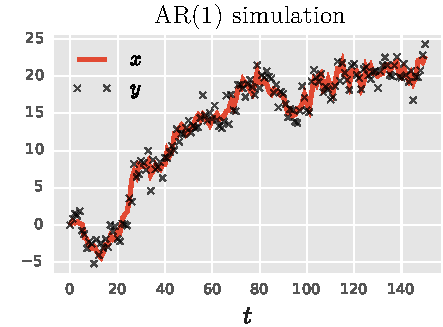
\includegraphics{img/ar1_ex_a}} 
%\newlength\graphicwidth
%\settowidth\graphicwidth{\mygraphic}
%\message{ar1 width \the\graphicwidth}

We begin with the background, where
SSMs are covered in necessary detail, Bayesian optimal filtering
and smoothing equations are derived and the role of the static parameters is elaborated
on. Following the background, in Section~\ref{sec:state_est} we focus on state estimation, first for linear
and then for nonlinear systems. The Kalman filter is introduced here as is the
concept of Gaussian filtering, a deterministic approximation used for nonlinear systems.
The fourth section is concerned with the two methods
of parameter estimation we are comparing: gradient based nonlinear optimization
and the Expectation Maximization (EM) algorithm. Our goal here is to present the underlying ideas,
the resulting equations and the most helpful literary references for one to be able to 
actually implement these methods.
 
The theoretical analysis is sufficiently detailed in order to 
draw some conclusions about the behavior of the
parameter estimation methods in the results section. The results section has two subsections: 
a target tracking application with simulated data and a biomedical signal processing 
application with real world data.



